\chapter{Background}

\section{Definitions}
\subsection{Epidemic and Pandemic }
An infectious disease is a disease that is caused by pathogenic micro organisms, such as bacteria, viruses, parasites or fungi; the diseases can be spread, directly or indirectly, from one person to another.An  epidemic is a situation where an infectious disease is affecting many people at a particular time and spread at a very high rate. A pandemic on the other is an epidemic over a large area \citep{morens2009pandemic}.

\subsection{deterministic and stochastic infectious disease models}
The dynamics of infectious disease propagation are modelled as dynamical system. A dynamical system is a system that evolves with time over a state space according to a fixed rule. Thus let $\mathbb{X}$ be a state space $\mathbb{T}$ set of times and $\mathbb{R}$ rule that specifies how the state evolves with time. the rule is a function that whose domain is $\mathbb{X} \mathbb{T}$ and co domain $\mathbb{X}$ that is,
\begin{equation*}
\mathbb{R}: \mathbb{X} \mathbb{T} \longrightarrow \mathbb{X}.
\end{equation*}

The population is characterized as $S(t)$, $E(t)$,$I(t)$ and $R(t)$ . Where $S(t)$ is the number of individuals susceptible but not infected at time $t$, $E(t)$ is the number of people exposed or infected but not infectious at time $t$, $I(t)$ is the number of infected and infectious people at time $t$ and $R(t)$ is the number of people removed from the ability of being infected.Removal is carried by either immunization,death,recovery from the disease. The epidemiological models can be classified as Susceptible,Infected and Recovered (SIR) , Susceptible Infected (SIS or SIS) , Susceptible -Exposed - Infectious and Removed (SEIR)  and any other intermediate category can be added.

The SIS model assumes that there is no immunity after recovery used to model infections where once a person recovers they become susceptible again for example infectious like flue. SIR model assumes that once a person recovers they become immune to the infection for example chicken pox. The SEIR assumes that onnce a person get becomes infected they do not  become infectious intermediately hence the intermediate compartment for exposed. 

The independent variable in the compartmental model is the time $t$ and the rates of transfer between compartments are expressed mathematically as a result models are formulated initially as differential equations. The most epidemic models are built on the SIR proposed by \cite{m1925applications}. The system can be written as;


\begin{center}
\begin{equation} \label{eqn1_1}
\left\lbrace \begin{array}{ccl}
\frac{dS}{dt} &= &-\alpha S_{(t)} I_{(t)},\\
 \frac{dI}{dt} &=& \alpha S_{(t)} I_{(t)} - \gamma  I_{(t)}, \\
 \frac{dR}{dt} &= &\gamma  I_{(t)},
\end{array} \right. 
\end{equation}
\end{center}

 with assumptions that there is homogeneous mixing in the population. That is the rate of new infections is proportional to the current numbers of susceptibles and infectives in the population. Which the main assumption deterministic models are built on. Deterministic population  models are models where the behaviour of the population of determined completely by history and the rules which govern the model. In formulating these models , in terms of derivatives of the sizes of the compartments and it is assumed that the number of members in each compartment is differentiable with time. This assumption is tenable only when the disease outbreak has been established  but not valid at the beginning of a disease out break when they are few infectives. When they are a few out breaks the number of infectious depends on random contacts of between small number of individuals.
 
 On the other hand Stochastic models are obtained by setting by adding a random variable called noise to the transmission dynamics of deterministic models.These random fluctuations may impact the evolution of the infection. Unlike deterministic model which assume homogeneous mix , an assumption which only holds in small populations. It is quiet unlikely that all people in will be equally susceptible to the disease and effective in spreading it \citep{ball1985deterministic}. A stochastic model can be further be described as a model in which the distribution of the length of the infectious period as allowed to have any distribution that can be describe by its Laplace transform \citep{addy1991generalized}.
 
 Lets an SIR compartmental model, for $t > 0$, $S(t),I(t),R(t)$ is the number of individuals in susceptible, infectious and removed. $N(t)$ the total number of particles at time $t$. The Poisson process, which is the underlying structure basic to the class of stochastic models and all Markov chain processes\citep{greenwood2009stochastic}. The individuals enter each compartment at random times and the initial fixed values , $S(0)$,$I(0)$ and $R(0)$ are fixed for some $\lambda > 0$. Letting $\beta$ to be the average number of  contacts an infectious person makes per unit of time that take leads to infection. The probability of a susceptible individual moving from compartment S to compartment I in the time interval $\left[ t,\triangle t \right]$ that is  S $\rightarrow S-1$ and I $\rightarrow I + 1 $ is $ \beta$ S I $ \triangle t + o (\triangle t)$. If it is assumed the an infected person recovers at the rate $\gamma$ hence the probability of an infected person moving from infected to recovered over an interval $\left[ t,\triangle t \right]$  given by $\gamma I_{t + \triangle t} -o (\triangle t)$ .It is known that,
 \begin{align*}
 N_t = S_t + I_t + R_t
 \\ \Rightarrow  R_t = N_t - S_t - I_t
\end{align*}  
Which implies that knowing $S_t,I_t$ is knowing $R_t$. Hence the model becomes an $S_t,I_t$ and thus the stochastic dynamical system can be written as;
 \begin{align}
 P((S_{t + \triangle t}, I_{t + \triangle t} - (S_t ,I_t) = ( - 1,1)) =  \beta S I  \triangle t + o (\triangle t).
 \\ P (((S_{t + \triangle t}, I_{t + \triangle t} - (S_t ,I_t) = ( 0,-1)) = \gamma I_{t + \triangle t} -o (\triangle t).
 \end{align}
\subsection{Network}


 A graph also known as a network   can be  defined as triple $G = (V,E,f)$ where $V$ is a finite set of nodes $E \subset V \oplus V = \left\lbrace e_1,e_2,\dots ,e_m \right\rbrace$ is a set and f is a mapping which associates some elements of $E$ to a pair of elements of $V$ \citep{estrada2012structure}. Nodes can be human beings, cities or houses while edges could be any connection such as friendship, physical connection or road.
 A network is said to be connected if they exist a path between any two nodes in the network.Distance between any two nodes in a network is defined as the length of the shortest path by each a node can be reached. This can be summed up as the average distance taken over all, pairs of individuals , which gives the idea of the typical distance between nodes in a network or the diameter of the graph which is the largest distance taken over all pairs.
 \subsection{Statistical Characterization}
 
 Networks can be characterized by the following statistical properties.
 \begin{itemize}
 \item[i] \textit{\textbf{Degree distribution}}
 The degree of a node is the number of connection a particular node  and is denoted as $k$  and the average distribution of a network is denoted by $<k>$. Looking at the entire space or network one can obtain a distribution for the degree. Let $n(k)$ be the number of nodes of degree $k$  in a network of size $n$, $p(k) = \dfrac{n(k)}{n}$. $p(k)$ represents the probability that a node selected uniformly at random  has degree $k$. the degree distribution is obtained by plotting $p(k)$ against $k$\citep{estrada2015first}. The common distribution found in network are normal distribution, exponential, power law distribution and poisson distribution.
 
   \citep{chung2002average}.
 \item[ii] \textit{\textbf{Clustering }}
 A cluster in a network  is a collection of nodes which are similar between them and are dissimilar to other nodes belonging to other clusters. Clustering in friendship network may mean friends people have in common. Local clustering in a network is measure by   the watts -stoggatz  coefficient and the global clustering by  Newman clustering coefficients.
 
 watts -stroggatz average clustering coefficient is given by 
 \begin{equation}
 \overline{C} = \dfrac{1}{n} \sum_i c_i
 \end{equation}
  $c_i = \dfrac{2t_i}{k_i(k_i-1)}$ where $t_i =$e number of triangles attached to node $i$ of degree $k_i$.
 
 The Newman clustering coefficient is given by
 \begin{equation}
 c = \frac{3t}{p_2} =\dfrac{3|c_3|}{p_2}
 \end{equation}
 where $t = c_3$ number of triangle in the network and $|p_2|$ the number of closed paths of length 2. 
 \end{itemize}
 \subsection{Random Graphs} A random graph can be defined as , given a $N$ number of vertices edges between them are drown such that between any pair $i,j$ there is an edge with uncorrelated probability $p$ \citep{newman2002random}. For example in \ref{fig:randomgraphs}, there are 3 random graphs with 10 vertices, with a probability of nodes $i,j$ being connect being 0, 0.5 and 0.8 in figure \ref{fig:a} \ref{fig:b} and \ref{fig:c} respectively. A random network model can exhibit the small world network property, it has an average degree $z= pN$. Random networks have a a low clustering coefficient $ c = \frac{z}{N}$ \citep{newman2003structure}.


\begin{figure}[h]
    \centering
    \begin{subfigure}[b]{0.3\textwidth}
        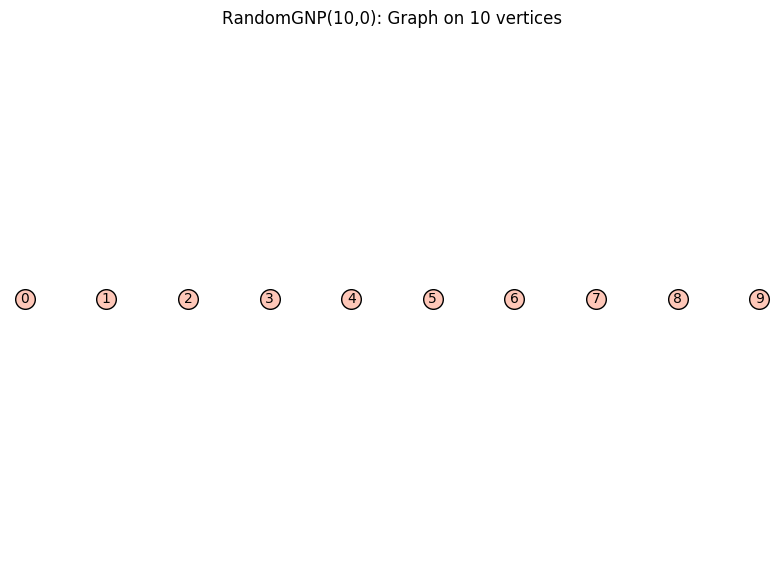
\includegraphics[scale=0.3]{images/rgraph2.png} 
        \caption{ $p =0$}
        \label{fig:a}
    \end{subfigure}
    ~ %add desired spacing between images, e. g. ~, \quad, \qquad, \hfill etc. 
      %(or a blank line to force the subfigure onto a new line)
    \begin{subfigure}[b]{0.3\textwidth}
        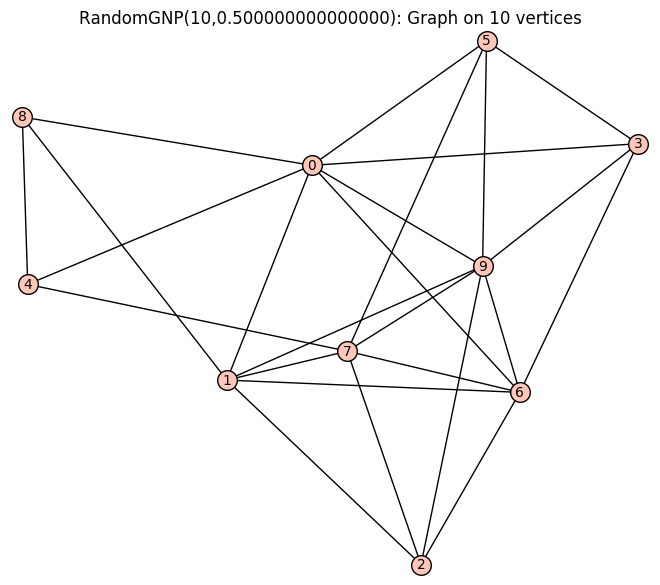
\includegraphics[width=\textwidth]{images/rgraph1.png}
        \caption{$p=0.5$}
        \label{fig:b}
    \end{subfigure}
    ~ %add desired spacing between images, e. g. ~, \quad, \qquad, \hfill etc. 
    %(or a blank line to force the subfigure onto a new line)
    \begin{subfigure}[b]{0.3\textwidth}
        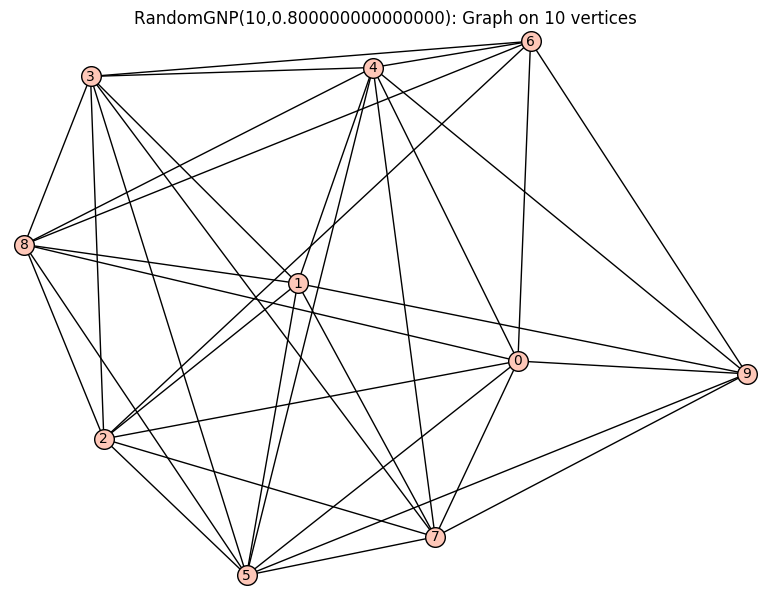
\includegraphics[width=\textwidth]{images/rgraph3}
        \caption{$p= 0.8$}
        \label{fig:c}
    \end{subfigure}
    \caption{Random Graphs}\label{fig:randomgraphs}
\end{figure}




Regular lattices and random graphs have a long history of use in network theory and to model population structures,\cite{harris1974contact}  gives an example of classic lattice. Models built on latices assume that individuals are located as nodes on a regular lattice and connections are made of some collection of near neighbours or each node. For example people may be spread out such that connections are made to their four nearest neighbours, one on the left,right, up and down this is called a Neuman neighbours  or eight neighbours where four diagonal elements are added to the Neuman neighbours and this is called the Moore neighbour hood \citep{lloyd2006infection}.To avoid the effect of the nodes at the end not being connected the last and first neighbours are made neighbours.

The main difference between a random graph and lattices is that interactions are local, that is individuals are only related to their neighbours. Where as in random networks the connections are made are global, that is connections are made without taking spatial locations of an individual into consideration. 


Small world networks  were first introduced by Watts and Strogatz as an intermediate between the regular lattice and randomly rewiring certain proportions $p$ of the network links\citep{watts1998collective}. The small world networks allows for random contacts across the network. That is in addition to near neighbours as in a regular lattice, each node has a random distant neighbour connected to it \citep{watts1998collective}.

 
  